\def\ACCOMPLETE{}
\ifdefined\COMPLETE
\else
\documentclass[12pt]{article}
\usepackage{amsmath,amssymb,amstext,amsthm} 
\usepackage[boxruled]{algorithm2e}
\usepackage{tikz}
\usepackage[inline]{enumitem}

\newcommand{\mc}{\mathcal}
\newcommand{\mb}{\mathbf}
\DeclareMathOperator*{\argmin}{arg\,min}
\DeclareMathOperator*{\argmax}{arg\,max}

\newtheorem{theorem}{Theorem}
\newtheorem{lemma}[theorem]{Lemma}
\newtheorem{definition}[theorem]{Definition}
\newtheorem{proposition}[theorem]{Proposition}
\newtheorem{corollary}[theorem]{Corollary}

\usetikzlibrary{shapes, calc, arrows, through, intersections, decorations.pathreplacing, patterns}

\begin{document}
\fi

Clustering is an under-specified task. Given a dataset, there is no unique or `correct' solution. The solution of choice varies with the intended application. In the absence of knowledge of the desired application, clustering problem is usually not well-defined. We need to incorporate domain expertise to better define the clustering problem. At the same time, performing clustering under many natural models of computation is computationally intractable. 

In this chapter, we take a new approach to alleviate these two issues in clustering. We first allow the clustering algorithm to be semi-supervised (through access to answers of natural queries). This makes the clustering problem better defined. We then ask the following question. \textit{Can semi-supervision help relax the computational burden of clustering?}

Aside from trial and error, one principled approach to supervision in clustering is through \textit{link/do-not-link} constraints \cite{basu2002semi,basu2004probabilistic, kulis2009semi}. In this case, besides the usual input, the clustering algorithm also receives a set of pairs which should always share the same cluster and a set of pairs which should always be separated into different clusters. Our approach combines the user-friendliness of link/do-not-link constraints with the advantages of interactiveness. We call it \textit{same-cluster} queries.  That is, the algorithm can interact with a domain expert (or an oracle) by asking whether two elements belong to the same cluster or not. The oracle responds by answering `yes' or `no' depending upon whether the two points share a cluster or are separated into different clusters. 

The general setting in this chapter is the following. Let $X$ be a set of elements that should be clustered and $d$ a distance metric over it. The oracle (e.g., a domain expert) has information about a target clustering $C^*$ in its mind. That target clustering satisfies some predefined clusterability condition (which we call $\gamma$-margin). The notion says that each cluster center is $\gamma$ times closer to the points in its own cluster than to points in different clusters. The clustering algorithm has access to $(X, d)$ and can also ask same-cluster queries about $C^*$. The goal of the algorithm is to efficiently recover the target clustering $C^*$ while making a `small' number of same-cluster queries to the oracle. 

We provide a polynomial time algorithm for clustering with queries, that succeeds (with high probability) under the assumption that the input satisfies the $\gamma$-margin condition for $\gamma > 1$. This algorithm makes $O\big(k^2\log k + k\log n)$ same-cluster queries to the oracle and runs in $O\big(kn\log n)$ time, where $k$ is the number of clusters and $n = |X|$.

We also consider the following special case. The target $C^*$ (in the oracle's mind) is the optimal solution of the $k$-means clustering problem and also satisfies the clusterability condition. In this case, the query-based algorithm succeeds with high probability as long as $\gamma >1$.  On the other hand, we show that without access to a same-cluster oracle, $k$-means clustering is NP-hard even when the optimal solution satisfies $\gamma$-margin property for $\gamma=\sqrt{3.4} \approx 1.84$ and $k=\Theta(n^\epsilon)$ (for any $\epsilon\in (0,1)$). This shows that access to a small number of same-cluster queries can provide an efficient algorithm for an otherwise NP-hard problem. This is an interesting trade-off between query complexity and computational complexity in the clustering domain. 

\section{Related Work}
This work combines two directions of research. The first is clustering under semi-supervision and the second is computational complexity of clustering. 

The most common framework to convey supervision in clustering is through a set of link/do-not-link constraints \cite{basu2002semi,basu2004probabilistic, kulis2009semi}. Here, the clustering algorithm is provided a list of pairs which should share the same cluster and a list of pairs which should be separated into different clusters. Here, the supervision is non-interactive. On the interactive side, Balcan et. al \cite{balcan2008clustering} introduced the notion of \textit{split/merge} queries. In their framework, the domain expert (or oracle) receives a clustering of the given dataset. Given a clustering, the oracle responds by suggesting either to merge two clusters or to split a cluster. For each query, the oracle should evaluate a clustering of the entire dataset. Another example of supervision is clustering was introduced by Ashtiani and Ben-David \cite{ashtiani2015representation}. Here, the oracle receives a small subset of the dataset and responds by outputting the `correct' clustering of that subset. Our approach combines the user-friendliness of link/do-not-link constraints (as opposed to requiring the oracle to answer queries about the whole data set or to cluster subsets of the data) with the advantages of interactiveness. 

The computational complexity of clustering is very well studied problem. Clustering is usually posed as an optimization problem where the goal is to minimize a given objective (or cost) function. $k$-means and $k$-median are two popular objective functions. However, many of the results are negative. For example, minimizing the $k$-means objective is NP-hard. Moreover, it is NP-Hard even for $k=2$ \cite{dasgupta2008hardness}, or even in a two-dimensional plane \cite{vattani2009hardness,mahajan2009planar}. Similarly, minimizing the $k$-median objective is also NP-Hard. Despite these negative results, clustering algorithms are routinely and successfully applied in practice. To explain this gap between theory and practice, notions of data niceness under which clustering becomes easy have been considered. The hypothesis is that real-world datasets are not worst-case and often have nice properties which makes clustering tractable. \cite{Ben-David15} has an extensive survey of such notions.

The notion of $\alpha$-center proximity introduced by Awasthi et. al \cite{awasthi2012center} is most related to our notion of margin (a comparison between the two can be found in Appendix \ref{appendix:gammaMrginVsAlphaCenter}). In the restricted scenario (i.e., when the centers of clusters are selected from the data set), their algorithm efficiently recovers the target clustering for $\alpha > 3$.  Balcan and Liang \cite{balcan2012clustering} provide a different algorithm and prove that recovery is possible for $\alpha > \sqrt{2} + 1$. Ben-David and Reyzin \cite{ben2014data} show that this problem is NP-Hard for $\alpha < 2$. Variants of these proofs for our $\gamma$-margin condition yield the feasibility of $k$-median clustering (centers of clusters are selected from the input) when the input satisfies the condition with $\gamma >2$ and NP hardness when $\gamma <2$.


\section{Problem Formulation}

Let $X$ be a subset of some Euclidean space, $\mb{R}^d$. A $k$-clustering of the set $X$ partitions it into $k$ disjoint subsets $\mc C = \{C_1, \ldots, C_k\}$. We say $x_1 \overset{C}{\sim} x_2$ if $x_1$ and $x_2$ belong to the same cluster according to $C$. Also, $n := |X|$. We say that a clustering $C$ is \emph{center-based} if there exists centers $\mu = \{\mu_1, \ldots, \mu_k\} \subset \mb R^d$ such that $C$ corresponds to the Voronoi diagram over these centers. Namely, for every $x$ in $X$ and $i \leq k$,  $x\in C_i \Leftrightarrow i=\argmin_j d(x,\mu_j)$. 


Next, we introduce our data niceness property or our notion of clusterability of a data set.

\begin{definition}[$\gamma$-margin]
\label{defn:alphacp}
Let $X$ be set of points in a metric space $(M, d)$. Let $C = \{C_1, \ldots, C_k\}$ be a center-based clustering of $X$ induced by centers $\mu_1, \ldots, \mu_k \in M$. We say that $C$ satisfies the $\gamma$-margin property if the following holds. For all $i \in [k]$ and every $x \in C_i$ and $y \in X \setminus C_i$,

$$\gamma d(x, \mu_i) < d(y, \mu_i)$$
\end{definition}


We now introduce our notion of a same-cluster oracle and same-cluster queries. For a clustering $C^*=\{ C^*_1, \ldots C^*_k\}$, a $C^*$-oracle is a function ${\mc O} : X \rightarrow \{true, false\}$ that answers queries according to $C^*$. We can think of the oracle as a human or domain-expert that has knowledge about the desired clustering and can answer the clustering algorithm's queries. The clustering algorithm then tries to recover $C^*$ by querying $\mc O$.

\begin{definition}[Same-cluster Query]
Given a clustering instance $X$ and a $C^*$-oracle $\mc O$. A same-cluster query asks whether two instances $x_1$ and $x_2$ belong to the same cluster, i.e., 
$$\mc O(x_1, x_2) = \left\{
	\begin{array}{ll}
		\mbox{true }  & \mbox{if } x_1 \overset{C^*}{\sim} x_2   \\
		\mbox{false } & o.w. 
	\end{array}
\right. $$
\end{definition}

\section{Clustering using same-cluster queries}
\label{section:clusteringWithQuery}

In this section we provide an efficient algorithm for clustering with queries. The setting is the one described in the previous section. In particular, it is assumed that the oracle has a center-based clustering in his mind which satisfies the $\gamma$-margin property. The space is Euclidean and the center of each cluster is the center of mass of the instances in that cluster. The algorithm not only makes same-cluster queries, but also another type of query defined as below.% queiries to the oracle, but this can be translated to binary same-cluster queries 


\begin{definition}[Cluster-assignment Query]
A cluster-assignment query asks the cluster index that an instance $x$ belongs to. In other words ${\mc O_{C^*}}(x) = i$ if and only if $x \in C^*_i$.
\end{definition}

Note however that each cluster-assignment query can be replaced with $k$ same-cluster queries (see appendix \ref{appendix:diffQueryModels}). Therefore, we can express everything in terms of the more natural notion of same-cluster queries, and the use of cluster-assignment query is just to make the representation of the algorithm simpler.

Our algorithm works in two phases. In the first phase, it approximates the center of one of the clusters. It does this by asking cluster-assignment queries about a set of points sampled uniformly at randomly, until it has a sufficient number of points from at least one cluster (say $C_p$). It uses the mean of these points $\mu_p^\prime$ as an approximation of the true cluster center $\mu_p$. 

In the second phase, the algorithm recovers all of the instances belonging to $C_p$. In order to do that, it first sorts all of the instances based on their distance to $\mu_p^\prime$. The margin assumption ensures that all of the points in $C_p$ lie inside a sphere centered at $\mu_p^\prime$ (which does not include points from any other cluster). It then tries to find the radius of this sphere by doing binary search using same-cluster queries. After that, the elements in $C_p$ will be located and can be removed from the data set. The algorithm repeats this process $k$ times to recover all of the clusters. The details of our approach is in Algorithm \ref{alg:steinerQueryPositive}. Note that $\beta$ is a small constant\footnote{It corresponds to the constant appeared in generalized Hoeffding inequality bound, discussed in Theorem \ref{thm:genHoeff} in appendix \ref{appendixsection:conIneq} }. 

\RestyleAlgo{boxruled}
\SetAlgoNoLine
\begin{algorithm}[!th]
 \caption{Algorithm for $\gamma(> 1)$-margin instances with queries}
 \label{alg:steinerQueryPositive}
 \KwIn{Clustering instance $X$, a $C^*$-oracle $\mc O$, the number of clusters $k$ and a parameter $\delta \in (0, 1)$}
 \KwOut{A clustering $C$ of the set $X$}

 \vspace{0.5em} $C = \{\}$, $S = X$ and $\eta = \beta \frac{\log k + \log(1/\delta)}{(\gamma-1)^4}$\\
 \While{$S \neq \phi$}{
 	\vspace{0.5em}\textbf{Phase 1}\\
 	Let $l = k \eta + 1$\\
	Draw $l$ points from $S$ uniformly at random\\
	Let $S_t = \{x \in S : {\mc O}(x)= t\}.$ where the oracle answers cluster-assignment queries about the members of $S$\\
    $p = \argmax_t |S_t|$ and $\mu_p' := \frac{1}{|S_p|}\sum_{x \in S_p} x$.\\

	\vspace{0.5em}\textbf{Phase 2}\\
    Sorts elements of $\{x: x\in S\}$ in increasing order of $d(x, \mu_p')$.\\    
    Binary search over $S$, to find $i$ such that $b_{i} \in C_p$ and $b_{i+1} \not\in C_p$. (This step involves making same-cluster queries to the oracle $\mc O$).\\ %We will later prove that $d(b_{idx}, c_p') = \max_{x \in C_p}d(x, c_p')$.
	$C_p' = \{x \in S: d(x, \mu_p') \le d(b_i, \mu_p')\}$.\\
	Delete $C_p'$ from $S$ and $C = C \cup \{C_p'\}$
 }
\end{algorithm}

Theorem \ref{thm:steinerQueryPositive} shows that if $\gamma > 1$ then our algorithm recovers the target clustering with high probability. Next, we give bounds on the time and query complexity of our algorithm. Theorem \ref{thm:steinerQueryPositiveComplexity} shows that our approach needs $O(k\log n + k^2\log k)$ queries and runs with time complexity $O(kn\log n)$.




\begin{lemma}
\label{lemma:hasGammaMargin}
Given a clustering instance $X \subseteq \mb R^d$. Let $C = \{C_1, \ldots, C_k\}$ be any center-based clustering of $X$ that satisfies the $\gamma$-margin property. Let $\mu_i$ be the set of centers corresponding to the centers of mass of $C_i$. Let $\mu_i'$ be such that $d(\mu_i, \mu_i') \le r(C_i)\epsilon$, where $r(C_i) = \max_{x\in C_i}d(x, \mu_i)$ . If $\gamma \ge 1 + 2\epsilon$ then 
$$\forall x \in C_i, \forall y \in {X} \setminus C_i \Rightarrow d(x, \mu_i') < d(y, \mu_i')$$
\end{lemma}

\begin{proof}
Fix any $x \in C_i$ and $y \in C_j$. $d(x, \mu_i') \le d(x, \mu_i)+d(\mu_i, \mu_i') \le r(C_i) (1+\epsilon)$. Similarly, $d(y, \mu_i') \ge d(y, \mu_i) - d(\mu_i, \mu_i') > (\gamma -\epsilon)r(C_i)$. Combining the two, we get that $d(x, \mu_i') < \frac{1+\epsilon}{\gamma-\epsilon}d(y, \mu_i')$. 
\end{proof}

\begin{lemma}
\label{lemma:phase1}
Let the framework be as in Lemma \ref{lemma:hasGammaMargin}. Let $S_p, C_p, \mu_p$, $\mu_p^\prime$ and $\eta$ be defined as in Algorithm \ref{alg:steinerQueryPositive}, and $\epsilon = \frac{\gamma - 1}{2}$. If $|S_p| > \eta$, then the probability that $d(\mu_p, \mu_p^\prime) > r(C_p)\epsilon$ is at most $\frac{\delta}{k}$.
\end{lemma}
\begin{proof}
Define a uniform distribution $U$ over $C_p$. Then $\mu_p$ and $\mu_p^\prime$ are the true and empirical mean of this distribution. Using a standard concentration inequality (Thm. \ref{thm:genHoeff} from Appendix \ref{appendixsection:conIneq}) shows that the empirical mean is close to the true mean, completing the proof. 

\end{proof}

\begin{theorem}
\label{thm:steinerQueryPositive}
Given a clustering instance $X \subseteq \mb R^d$. Let $C^* = \{C_1^*, \ldots, C_k^*\}$ be center-based clustering of $X$ that satisfies the $\gamma$-margin property. Given $\delta \in (0, 1)$ and $\gamma > 1$ and a $C^*$-oracle, with probability at least $1-\delta$, Algorithm \ref{alg:steinerQueryPositive} outputs $C^*$.
\end{theorem}

\begin{proof}
In the first phase of the algorithm we are making $l>k\eta$ cluster-assignment queries. Therefore, using the pigeonhole principle, we know that there exists cluster index $p$ such that $|S_p| > \eta$. Then Lemma \ref{lemma:phase1} implies that the algorithm chooses a center $\mu_p^\prime$ such that with probability at least $1-\frac{\delta}{k}$ we have $d(\mu_p, \mu_p^\prime) \le r(C_p)\epsilon$. By Lemma \ref{lemma:hasGammaMargin}, this would mean that $d(x, \mu_p^\prime) < d(y, \mu_p')$ for all $x \in C_p$ and $y \not\in C_p$. Hence, the radius $r_i$ found in the phase two of Alg. \ref{alg:steinerQueryPositive} is such that $r_{i} = \max\limits_{x \in C_p} d(x, \mu_p^\prime)$. This implies that $C_p^\prime$ (found in phase two) equals to $C_p$. Hence, with probability at least $1-\frac{\delta}{k}$ one iteration of the algorithm successfully finds all the points in a cluster $C_p$. Using union bound, we get that with probability at least $1-k\frac{\delta}{k} = 1-\delta$, the algorithm recovers the target clustering.
\end{proof}

\begin{theorem}
\label{thm:steinerQueryPositiveComplexity}
Let the framework be as in theorem \ref{thm:steinerQueryPositive}. Then Algorithm \ref{alg:steinerQueryPositive} 
\begin{itemize}[nolistsep,noitemsep]
\item Makes $O\big(k\log n + k^2\frac{\log k + \log (1/\delta)}{(\gamma - 1)^4}\big)$ same-cluster queries to the oracle $\mc O$.
\item Runs in $O\big(kn\log n + k^2\frac{\log k + \log (1/\delta)}{(\gamma - 1)^4}\big)$ time.
\end{itemize}
\end{theorem}

\begin{proof}
In each iteration (i) the first phase of the algorithm takes $O(\eta)$ time and makes $\eta+1$ cluster-assignment queries (ii) the second phase takes $O(n\log n)$ times and makes $O(\log n)$ same-cluster queries. Each cluster-assignment query can be replaced with $k$ same-cluster queries; therefore, each iteration runs in $O(k\eta + n\log n)$ and uses $O(k\eta + \log n)$ same-cluster queries. By replacing $\eta = \beta\frac{\log k + \log(1/\delta)}{(\gamma-1)^4}$ and noting that there are $k$ iterations completes the proof.
\end{proof}

\section{Hardness of $k$-means with Margin}
\label{section:lowerBounds}

Finding $k$-means solution without the help of an oracle is generally computationally hard. In this section, we will show that solving Euclidean $k$-means remains hard even if we know that the optimal solution satisfies the $\gamma$-margin property for $\gamma=\sqrt{3.4}$. In particular, we show the hardness for the case of $k=\Theta(n^\epsilon)$ for any $\epsilon\in (0,1)$.

%This is a critical result for our purpose, because it shows that our niceness assumption (i.e., the $\gamma$-margin property) is not too strong, and the use of oracle is necessary.

In Section \ref{section:clusteringWithQuery}, we proposed a polynomial-time algorithm that could recover the target clustering using $O(k^2\log k +k\log n)$ queries, assuming that the clustering satisfies the $\gamma$-margin property for $\gamma>1$. Now assume that the oracle conforms to the optimal $k$-means clustering solution. In this case, for $1<\gamma\le \sqrt{3.4} \approx 1.84$, solving $k$-means clustering would be NP-hard without queries, while it becomes efficiently solvable with the help of an oracle \footnote{To be precise, note that the algorithm used for clustering with queries is probabilistic, while the lower bound that we provide is for deterministic algorithms. However, this implies a lower bound for randomized algorithms as well unless $BPP\neq P$}. 

Given a set of instances $\mc X \subset \mb R ^d$, the $k$-means clustering problem is to find a clustering $\mc C = \{C_1, \ldots, C_k\}$ which minimizes $f(\mc C) = \sum\limits_{C_i} \min\limits_{\mu_i\in {\mb R}^d}\sum\limits_{x\in C_i} \|x - \mu_i \|_2^2$. The decision version of $k$-means is, given some value $L$, is there a clustering $\mc C$ with cost $\le L$? The following theorem is the main result of this section. 

\begin{theorem}
\label{thm:gammaLower}
Finding the optimal solution to Euclidean $k$-means objective function is NP-hard when $k=\Theta(n^\epsilon)$ for any $\epsilon \in (0,1)$, even when the optimal solution satisfies the $\gamma$-margin property for $\gamma = \sqrt{3.4}$.
\end{theorem}

This results extends the hardness result of \cite{ben2014data} to the case of Euclidean 
metric, rather than arbitrary one, and to the $\gamma$-margin condition (instead of the $\alpha$-center proximity there). In the next sections, we provide an outline of the proof. Some of the missing details can be found in the appendix (\ref{appendix:lowerBoundProof}).

\subsection{Overview of the proof}

Our method to prove Thm. \ref{thm:gammaLower} is based on the approach employed by \cite{vattani2009hardness}. However, the original construction proposed in \cite{vattani2009hardness} does not satisfy the $\gamma$-margin property. Therefore, we have to modify the proof by setting up the parameters of the construction more carefully. 

To prove the theorem, we will provide a reduction from the problem of Exact Cover by 3-Sets (\textsc{X3C}) which is NP-Complete \cite{garey2002computers}, to the decision version of $k$-means.
%(which given a real value $L$, asks whether a clustering with cost $\le L$ exists).

\begin{definition}[\textsc{X3C}]
Given a set $U$ containing exactly $3m$ elements and a collection $\mc S = \{S_1, \ldots, S_l\}$ of subsets of $U$ such that each $S_i$ contains exactly three elements, does there exist $m$ elements in $\mc S$ such that their union is $U$? 
\end{definition}

We will show how to translate each instance of X3C, $(U,\mc S)$, to an instance of $k$-means clustering in the Euclidean plane, $X$. In particular, $X$ has a grid-like structure consisting of $l$ rows (one for each $S_i$) and roughly $6m$ columns (corresponding to $U$) which are embedded in the Euclidean plane. The special geometry of the embedding makes sure that any low-cost $k$-means clustering of the points (where $k$ is roughly $6ml$) exhibits a certain structure. In particular, any low-cost $k$-means clustering could cluster each row in only two ways; One of these corresponds to $S_i$ being included in the cover, while the other means it should be excluded. We will then show that $U$ has a cover of size $m$ if and only if $X$ has a clustering of cost less than a specific value $L$. Furthermore, our choice of embedding makes sure that the optimal clustering satisfies the $\gamma$-margin property for $\gamma=\sqrt{3.4} \approx 1.84$.

  \begin{figure}[!tbp]
  \centering
  \begin{minipage}[b]{0.49\textwidth}
    \resizebox{\linewidth}{!}{\ifdefined\ACCOMPLETE
\else
\documentclass[12pt]{article}
\usepackage{tikz}
\usetikzlibrary{shapes, calc, arrows, through, intersections, decorations.pathreplacing, patterns}

\begin{document}
\fi
\def\alph{$2+\sqrt{5}$}
\begin{tikzpicture}[scale=7]

	\node[label=180:$R_1$] at (0.0,0) {$\diamond$};	
	\node[] at (0.1,0) {$\bullet$};
	\node[] at (0.2,0) {$\bullet$};
	\node[] at (0.3,0) {$\bullet$};
	\node[] at (0.4,0) {$\bullet$};
	\node[] at (0.6,0) {$\ldots$};
	
	\node[] at (0.8,0) {$\bullet$};
	\node[] at (0.9,0) {$\bullet$};
	\node[] at (1.0,0) {$\diamond$};
	
	
	\node[label=180:$G_1$] at (0.0,-0.1) {};	
	\node[] at (0.2,-0.1) {$\circ$};
	\node[] at (0.4,-0.1) {$\circ$};
	\node[] at (0.6,-0.1) {$\ldots$};
	
	\node[] at (0.8,-0.1) {$\circ$};
	
	\node[label=180:$R_2$] at (0.0,-0.2) {$\diamond$};	
	\node[] at (0.1,-0.2) {$\bullet$};
	\node[] at (0.2,-0.2) {$\bullet$};
	\node[] at (0.3,-0.2) {$\bullet$};
	\node[] at (0.4,-0.2) {$\bullet$};
	\node[] at (0.6,-0.2) {$\ldots$};
	
	\node[] at (0.8,-0.2) {$\bullet$};
	\node[] at (0.9,-0.2) {$\bullet$};
	\node[] at (1.0,-0.2) {$\diamond$};
	
	
	
	\node[label=180:$G_{l-1}$] at (0.0,-0.4) {};	
	\node[] at (0.2,-0.4) {$\circ$};
	\node[] at (0.4,-0.4) {$\circ$};
	\node[] at (0.6,-0.4) {$\ldots$};
	
	\node[] at (0.8,-0.4) {$\circ$};
	
	\node[label=180:$R_l$] at (0.0,-0.5) {$\diamond$};	
	\node[] at (0.1,-0.5) {$\bullet$};
	\node[] at (0.2,-0.5) {$\bullet$};
	\node[] at (0.3,-0.5) {$\bullet$};
	\node[] at (0.4,-0.5) {$\bullet$};
	\node[] at (0.6,-0.5) {$\ldots$};
	
	\node[] at (0.8,-0.5) {$\bullet$};
	\node[] at (0.9,-0.5) {$\bullet$};
	\node[] at (1.0,-0.5) {$\diamond$};
	
	
	\node[label=90:\scriptsize$d$] at (0.05,0.0) {};
	\node[label=90:\scriptsize$2$] at (0.15,0.0) {};
	\node[label=90:\scriptsize$2$] at (0.85,0.0) {};
	\node[label={90:\scriptsize $d-\epsilon$}] at (0.97,0.0) {};
	\node[label=90:\scriptsize$4$] at (0.3,-0.1) {};
	
	
	\draw[<->] (0.02, 0.0) -- (0.08, 0.0);
	\draw[<->] (0.12, 0.0) -- (0.18, 0.0);
	\draw[<->] (0.82, 0.0) -- (0.88, 0.0);
	\draw[<->] (0.92, 0.0) -- (0.98, 0.0);
	

	\draw[<->] (0.38, -0.1) -- (0.22, -0.1);
\end{tikzpicture}


\ifdefined\ACCOMPLETE
\else
\end{document}
\fi
}
    \caption{Geometry of $H_{l,m}$. This figure is similar to Fig. 1 in \cite{vattani2009hardness}.  
    Reading from letf to right, each row $R_i$ consists of a diamond ($s_i$), $6m+1$ bullets ($r_{i,1},\ldots,r_{i,6m+1}$), and another diamond ($f_i$). Each rows $G_i$ consists of $3m$ circles ($g_{i,1}, \ldots, g_{i,3m}$).}
    \label{fig:lowerBoundComponent}
  \end{minipage}
  \hfill
  \begin{minipage}[b]{0.49\textwidth}
    \ifdefined\ACCOMPLETE
\else
\documentclass[12pt]{article}
\usepackage{tikz}
\usetikzlibrary{shapes, calc, arrows, through, intersections, decorations.pathreplacing, patterns}

\begin{document}
\fi
\def\alph{$2+\sqrt{5}$}
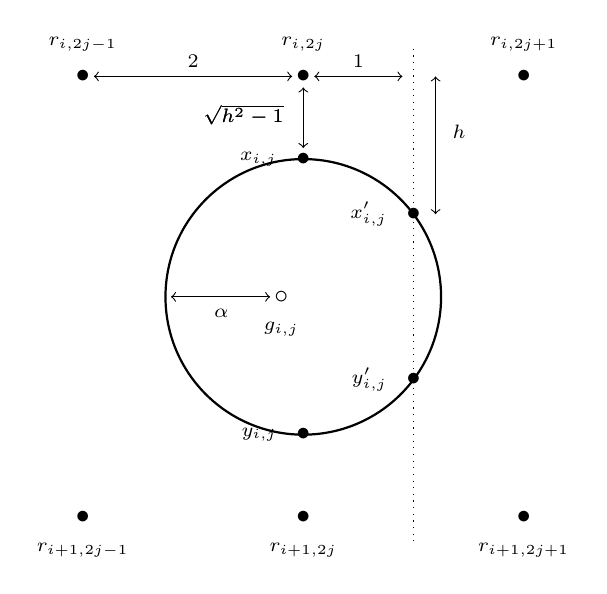
\begin{tikzpicture}[scale=7]

	
	\node[label=90:\scriptsize $r_{i,2j-1}$] at (0.1,0) {$\bullet$};
	\node[label=90:\scriptsize $r_{i,2j}$] at (0.5,0) {$\bullet$};
	\node[label=90:\scriptsize $r_{i,2j+1}$] at (0.9,0) {$\bullet$};
	
	\node[label=180:\scriptsize $\sqrt{h^2-1}$] at (0.5,-0.07) {};
	\node[label=180:\scriptsize $x_{i,j}$] at (0.5,-0.15) {$\bullet$};
	
	
	\node[label=180:\scriptsize $h$] at (0.83,-0.1) {};
	\node[label=180:\scriptsize $x_{i,j}'$] at (0.7,-0.25) {$\bullet$};
	
	\node[label=270:\scriptsize $g_{i,j}$] at (0.46,-0.4) {$\circ$};
	
	
	\node[label=180:\scriptsize $y_{i,j}$] at (0.5,-0.65) {$\bullet$};
	\node[label=180:\scriptsize $y_{i,j}'$] at (0.7,-0.55) {$\bullet$};
	
	
	\node[label=270:\scriptsize $r_{i+1,2j-1}$] at (0.1,-0.8) {$\bullet$};
	\node[label=270:\scriptsize $r_{i+1,2j}$] at (0.5,-0.8) {$\bullet$};
	\node[label=270:\scriptsize $r_{i+1,2j+1}$] at (0.9,-0.8) {$\bullet$};
	
	
	\node[label=180:\scriptsize $\sqrt{h^2-1}$] at (0.5,-0.07) {};
	
	
	\node[label=180:\scriptsize $\alpha$] at (0.4,-0.43) {};
	\node[label=90:\scriptsize $1$] at (0.6,-0.02) {};
	\node[label=90:\scriptsize $2$] at (0.3,-0.02) {};
	
	
	\draw[<->] (0.5,-0.13) -- (0.5,-0.02);
	\draw[<->] (0.26,-0.4) -- (0.44,-0.4);
	\draw[dotted,-] (0.7, 0.05) -- (0.7, -0.85);
	\draw[<->] (0.74, 0.0) -- (0.74, -0.25);
	\draw[<->] (0.68, 0.0) -- (0.52, 0.0);
	\draw[<->] (0.12, 0.0) -- (0.48, 0.0);
	\draw[black, thick] (0.5,-0.4) circle (0.25);
\end{tikzpicture}


\ifdefined\ACCOMPLETE
\else
\end{document}
\fi

    \caption{The locations of $x_{i,j}$, $x_{i,j}'$, $y_{i,j}$ and $y_{i,j}'$ in the set $Z_i$. Note that the point $g_{i,j}$ is not vertically aligned with $x_{i, j}$ or $r_{i, 2j}$. This figure is adapted from \cite{vattani2009hardness}.}
    \label{fig:ZFig}
  \end{minipage}
\end{figure}

\subsection{Reduction design}
Given an instance of X3C, that is the elements $U = \{1, \ldots, 3m\}$ and the collection $\mc S$, we construct a set of points $X$ in the Euclidean plane which we want to cluster. Particularly, $X$ consists of a set of points $H_{l,m}$ in a grid-like manner, and the sets $Z_i$ corresponding to $S_i$. In other words, $X = H_{l,m} \cup (\cup_{i=1}^{l-1} Z_i)$. 

The set $H_{l,m}$ is as described in Fig. \ref{fig:lowerBoundComponent}. The row $R_i$ is composed of $6m + 3$ points $\{s_i, r_{i, 1}, \ldots, r_{i, 6m+1}, f_i\}$. Row $G_i$ is composed of $3m$ points $\{g_{i,1}, \ldots, g_{i, 3m}\}$. The distances between the points are also shown in Fig. \ref{fig:lowerBoundComponent}. Also, all these points have weight $w$, simply meaning that each point is actually a set of $w$ points on the same location.

Each set $Z_i$ is constructed based on $S_i$. In particular, $Z_i = \cup_{j\in [3m]} B_{i,j}$, where $B_{i,j}$ is a subset of $\{x_{i,j},x_{i,j}',y_{i,j},y_{i,j}'\}$ and is constructed as follows: $x_{i,j} \in B_{i,j}$ iff $j \not\in S_i$, and $x_{i,j}' \in B_{i,j}$ iff $j \in S_i$. Similarly,  $y_{i,j} \in B_{i,j}$ iff $j \not\in S_{i+1}$, and $y_{i,j}' \in B_{i,j}$ iff $j \in S_{i+1}$. Furthermore, $x_{i, j}, x_{i,j}^\prime, y_{i,j}$ and $y_{i, j}^\prime$ are specific locations as depicted in Fig. \ref{fig:ZFig}. In other words, exactly one of the locations $x_{i,j}$ and $x_{i,j}^\prime$, and one of $y_{i,j}$ and $y_{i,j}^\prime$ will be occupied. We set the following parameters. 
\vspace{-0.1in}
\begin{align*}
&h = \sqrt{5}, d = \sqrt{6}, \epsilon = \frac{1}{w^2}, \lambda = \frac{2}{\sqrt{3}}h, k = (l-1)3m + l(3m+2)\\
& L_1 = (6m+3)wl, L_2 = 3m(l-1)w, L = L_1 + L_2 - m\alpha, \alpha = \frac{d}{w}-\frac{1}{2w^3}
\end{align*}


\begin{lemma}
\label{lemma:kmeansEquivalenceX3C}
The set $X = H_{l,n} \cup Z$ has a $k$-clustering of cost less or equal to $L$ if and only if there is an exact cover for the X3C instance.
\end{lemma}

\begin{lemma}
\label{lemma:gammaLower}
Any $k$-clustering of $X = H_{l,n} \cup Z$ with cost $\le L$ has the $\gamma$-margin property where $\gamma = \sqrt{3.4}$. Furthermore, $k = \Theta(n^{\epsilon})$.
\end{lemma}

The proofs are provided in Appendix \ref{appendix:lowerBoundProof}. Lemmas \ref{lemma:kmeansEquivalenceX3C} and \ref{lemma:gammaLower} together show that $X$ has a $k$-clustering of cost $\le L$ satisfying the $\gamma$-margin property (for $\gamma = \sqrt{3.4}$) if and only if there is an exact cover by $3$-sets for the X3C instance. This completes the proof of our main result (Thm. \ref{thm:gammaLower}). 

\section{Conclusions and Future Directions}
In this work we introduced a framework for semi-supervised clustering with same-cluster queries. Those queries can be viewed as a natural way for a clustering mechanism to gain domain knowledge, without which clustering is an under-defined task. The focus of our analysis was the computational and query complexity of %clustering in this  Then query complexity and computational complexity of 
such problems, when the input data set satisfies a clusterability condition -- the $\gamma$-margin property.

Our main result shows that access to a limited number of such query answers (logarithmic in the size of the data set and quadratic in the number of clusters) allows efficient successful clustering under conditions (margin parameter between 1 and $\sqrt{3.4} \approx 1.84$) that render the problem NP-hard without the help of such a query mechanism.  
 
With practical applications of clustering in mind, a natural extension of our model is to allow the oracle (i.e., the domain expert) to refrain from answering a certain fraction of the queries, or to make a certain number of errors in its answers. It would be interesting to analyze how the performance guarantees of query-based algorithms behave as a function of such abstentions and error rates. 

\ifdefined\COMPLETE
\else
\end{document}
\fi
